\title{Warm-Up for April 4th, 2022}
\author{Dr. Jordan Hanson - Whittier College Dept. of Physics and Astronomy}
\date{\today}
\documentclass[12pt]{article}
\usepackage[a4paper, total={18cm, 27cm}]{geometry}
\usepackage{graphicx}
\usepackage{amsmath}
\usepackage{bm}
\def\rcurs{{\mbox{$\resizebox{.16in}{.08in}{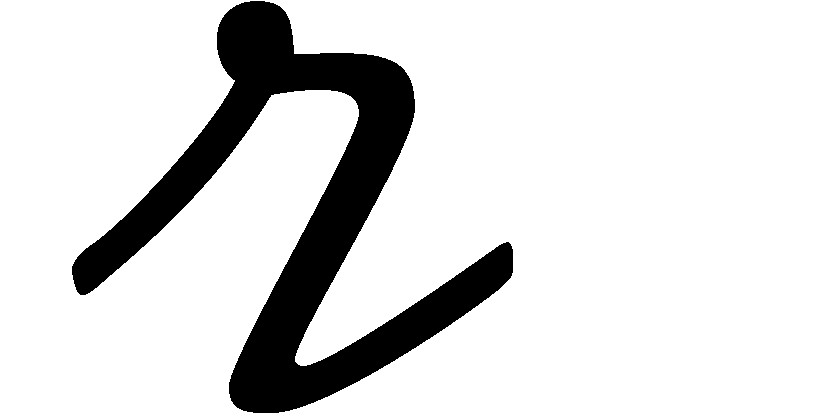
\includegraphics{ScriptR}}$}}}
\def\brcurs{{\mbox{$\resizebox{.16in}{.08in}{
\includegraphics{BoldR}}$}}}
\def\hrcurs{{\mbox{$\hat \brcurs$}}}
 
\begin{document}
\maketitle
\small
\section{Memory Bank}
\begin{enumerate}
\item Electric field and displacement in linear dielectric: $\mathbf{D} = \epsilon \mathbf{E}$.
\item Gauss' Law in dielectrics: $\oint \mathbf{D} \cdot d\mathbf{a} = Q_{\rm f, enc}$
\item Work, energy in dielectrics: $W = \frac{1}{2}\int \mathbf{D} \cdot \mathbf{E} ~ d\tau$
\item Relative permittivity: $\epsilon_r = \epsilon / \epsilon_0$
\end{enumerate}

\section{Work, Capacitance, and Energy in Matter}

\begin{enumerate}
\item Suppose the capacitor in Fig. \ref{fig:1} is filled with a linear dielectric with dielectric permittivity $\epsilon$.  Using the formulas in the memory bank, prove that the capacitance \textit{increases} to $C = \epsilon_r C$, relative to the air-filled capacitor.
\end{enumerate}

\begin{figure}
\centering
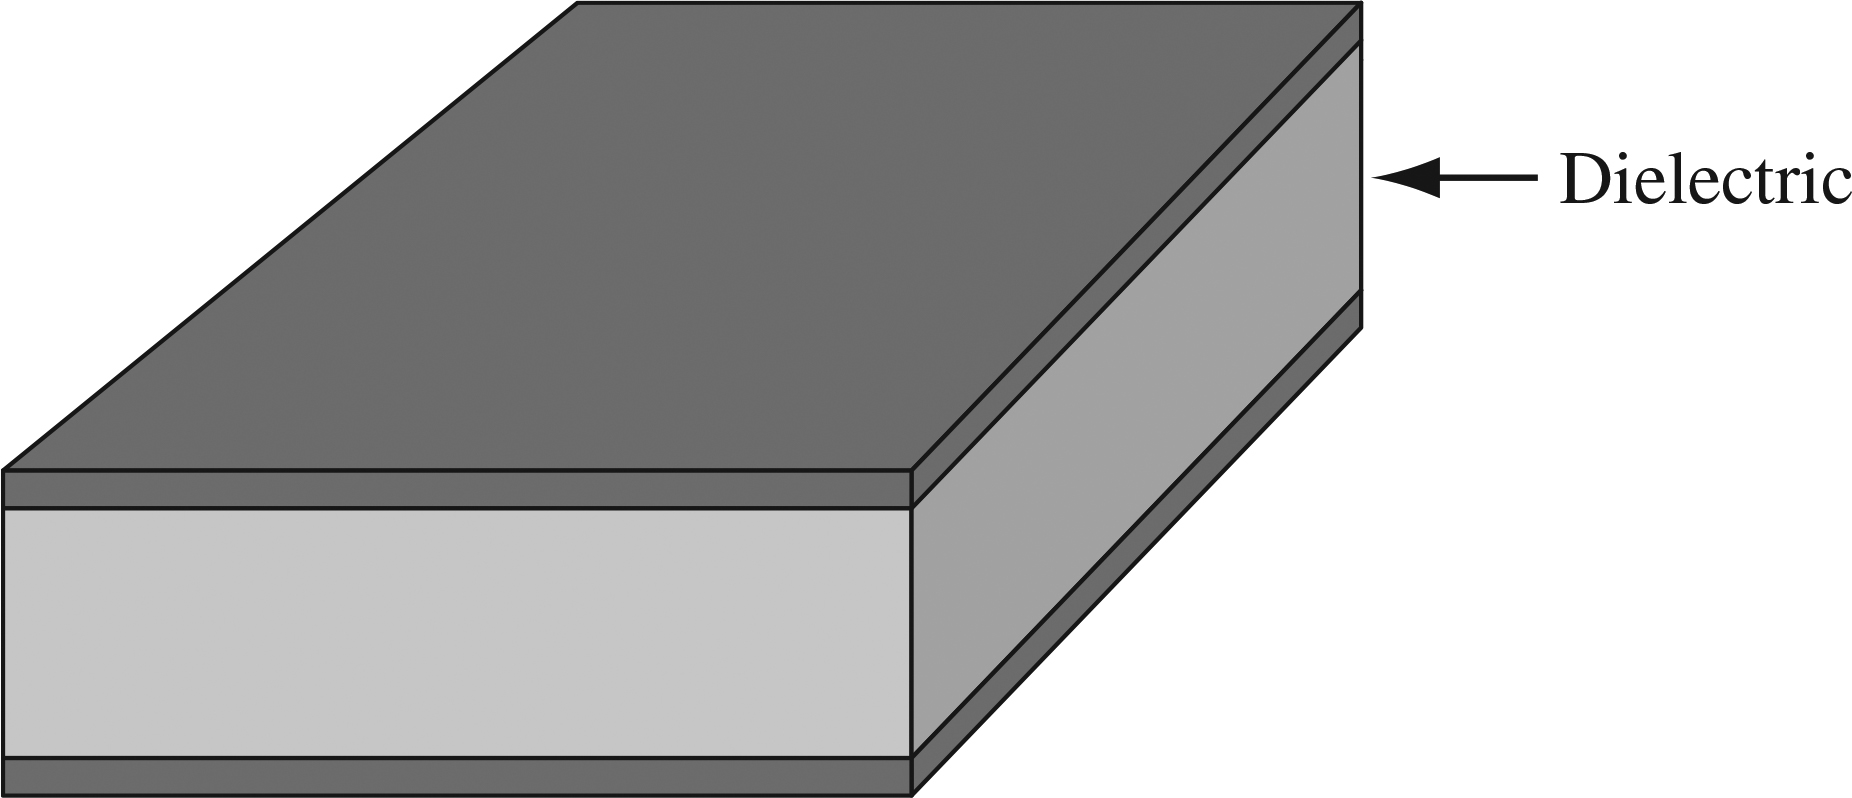
\includegraphics[width=0.4\textwidth]{figures/4_23.jpg}
\caption{\label{fig:1} A capacitor area $A$ and separation distance $d$ filled with dielectric.}
\end{figure}

\end{document}